\documentclass[10pt, a4paper, twocolumn]{article}

% --- UNIVERSAL PREAMBLE BLOCK ---
\usepackage[a4paper, top=2.0cm, bottom=2.5cm, left=1.5cm, right=1.5cm, columnsep=0.7cm]{geometry}
\usepackage{fontspec}
\usepackage[english, provide=*]{babel}

\babelprovide[import, onchar=ids fonts]{english}

% Fonts
\setmainfont{Noto Sans}
\setsansfont{Noto Sans}
\setmonofont{Noto Sans Mono}

% Packages for layout, math, and graphics
\usepackage{amsmath}
\usepackage{amssymb}
\usepackage{booktabs}
\usepackage{graphicx}
\usepackage{xcolor}
\usepackage{fancyhdr}
\usepackage{titlesec}
\usepackage{enumitem}
\usepackage{abstract}
\usepackage{hyperref}
\usepackage{listings}
\usepackage{algorithm}
\usepackage{algpseudocode}
\usepackage{caption}
\usepackage{float}
\usepackage{tikz} 

% --- BRANDING & STYLING ---
\definecolor{DeepBlue}{RGB}{12, 45, 72}
\definecolor{AccentBlue}{RGB}{46, 134, 193}
\definecolor{AlertRed}{RGB}{192, 57, 43}
\definecolor{CodeGray}{RGB}{245, 245, 245}
\definecolor{CodeGreen}{RGB}{0, 150, 0}
\definecolor{CodePurple}{RGB}{128, 0, 128}

% Hyperlink Setup
\hypersetup{
    colorlinks=true,
    linkcolor=DeepBlue,
    filecolor=AccentBlue,
    urlcolor=AccentBlue,
    citecolor=DeepBlue,
    pdftitle={Open Hallucination Index: Architectural Whitepaper},
    pdfauthor={Fabian Zimber}
}

% Header and Footer
\pagestyle{fancy}
\fancyhf{}
\fancyhead[L]{\footnotesize \textcolor{DeepBlue}{\textbf{Open Hallucination Index (OHI)}}}
\fancyhead[R]{\footnotesize \textit{Shiftbloom Studio}}
\fancyfoot[C]{\thepage}
\renewcommand{\headrulewidth}{0.4pt}
\renewcommand{\headrule}{\hbox to\headwidth{\color{AccentBlue}\leaders\hrule height \headrulewidth\hfill}}

% Title Formatting
\titleformat{\section}
  {\normalfont\Large\bfseries\color{DeepBlue}}{\thesection}{1em}{}
\titleformat{\subsection}
  {\normalfont\large\bfseries\color{DeepBlue}}{\thesubsection}{1em}{}
\titleformat{\subsubsection}
  {\normalfont\normalsize\bfseries\color{DeepBlue}}{\thesubsubsection}{1em}{}

% Listings configuration
\lstset{
    backgroundcolor=\color{CodeGray},
    commentstyle=\color{CodeGreen},
    keywordstyle=\color{CodePurple}\bfseries,
    numberstyle=\tiny\color{gray},
    stringstyle=\color{AlertRed},
    basicstyle=\ttfamily\footnotesize,
    breakatwhitespace=false,
    breaklines=true,
    captionpos=b,
    keepspaces=true,
    numbers=left,
    numbersep=5pt,
    showspaces=false,
    showstringspaces=false,
    showtabs=false,
    tabsize=2,
    frame=single,
    rulecolor=\color{gray!20}
}

% --- DOCUMENT META ---

\title{\vspace{-1em}\textbf{\Huge \textcolor{DeepBlue}{Open Hallucination Index (OHI)}}\\[0.5em] 
\Large \textit{A Sovereign Architectural Framework for Restoring Epistemic Integrity in the Era of Probabilistic Generative AI}}

\author{
    \textbf{Fabian Zimber} \\
    Lead Research Scientist, Shiftbloom Studio \\
    \texttt{fabian@shiftbloom.studio}
}

\date{\today}

\begin{document}

\twocolumn[
  \begin{@twocolumnfalse}
    \maketitle
    \begin{abstract}
      \noindent \textbf{Abstract:} The rapid adoption of Large Language Models (LLMs) has precipitated an epistemic crisis, characterized by the proliferation of "hallucinations"—synthetically generated statements that lack factual grounding. This paper introduces the Open Hallucination Index (OHI), a comprehensive architectural framework designed to transition the industry from "Generative AI" to "Verifiable AI." Unlike traditional Retrieval-Augmented Generation (RAG), which remains susceptible to the stochastic nature of the generator, OHI establishes a deterministic "Trust Layer" that operates post-generation. By leveraging \textit{Claim Decomposition}, a hybrid \textit{GraphRAG} approach utilizing Neo4j and Qdrant, and the standardized \textit{Model Context Protocol (MCP)}, OHI provides a quantifiable, audit-proof metric for truth. We present a reference implementation demonstrating local sovereignty using vLLM, detail the algorithmic rigor of the \textit{Hybrid Verification Oracle}, and analyze the system's performance in handling high-throughput verification tasks without reliance on proprietary black-box models.
      \vspace{2.5em}
    \end{abstract}
  \end{@twocolumnfalse}
]

\section{Introduction: The Epistemic Deficit}

\subsection{The Ontology of Stochastic Fabulation}
The current technological landscape is marked by a fundamental disruption in the production and distribution of knowledge. With the ubiquitous spread of Large Language Models (LLMs), the paradigm of information genesis has shifted from the deterministic querying of curated databases to probabilistic synthesis. While this shift has unlocked unprecedented capabilities in generating natural language, it confronts society with an epistemological crisis: the erosion of factual truth through "hallucinations."

As noted by Bender et al. in their seminal work on "Stochastic Parrots" \cite{bender2021}, LLMs operate as statistical pattern recognition systems that learn probability distributions over token sequences without a referential anchoring in extra-linguistic reality. They mimic the discourse of truth without having access to truth itself. This decoupling of form from content is an inherent feature of the Transformer architecture, optimized for plausibility rather than veracity. In critical domains such as jurisprudence, medicine, and engineering, the cost of such "stochastic integrity" is prohibitive.

\subsection{Epistemic Vigilance and the Trust Dilemma}
The necessity of a verification framework arises not only from technical deficits but from the psychological interaction between humans and machines. Cognitive science suggests that users tend to attribute an undeserved "epistemic authority" to AI systems. Jäger \cite{jaeger2024} defines this as a functional role based on the attribution of competence and reliability. LLMs simulate this competence through linguistic fluency, leading to "automation bias"—the tendency to trust algorithmic decisions even in the face of contradictory evidence.

Furthermore, "deferred trust" occurs when users shift their epistemic dependency from perceived biased human sources to AI systems, which are falsely viewed as neutral actors. While studies show an epistemic bias in favor of AI in factual domains, this trust is "brittle"; a single obvious error can collapse the entire system's credibility once "epistemic vigilance" is reactivated. OHI aims to institutionalize this vigilance technically.

\subsection{Political Sovereignty and Proprietary Biases}
A critical dimension of the hallucination debate is the political nature of the "truth" generated by LLMs. Proprietary models (Closed Source) undergo opaque Reinforcement Learning from Human Feedback (RLHF) processes, which inevitably encode the ideological, cultural, and political biases of their developers. Studies have shown significant ideological skewing in models like GPT-4, often favoring specific worldviews or failing systematically on sensitive topics.

In this context, hallucination becomes a political problem: if a model fabricates facts that correspond with embedded biases, disinformation is scaled. OHI addresses this through "local sovereignty." By utilizing open architectures (Open Source models like Qwen, local knowledge graphs), organizations can reclaim sovereignty over the "Ground Truth." Instead of relying on a model trained in California to know the laws of another nation, OHI enforces validation against a locally controlled data basis.

\subsection{The Failure of Naive RAG}
Retrieval-Augmented Generation (RAG) was proposed to ground LLM responses in retrieved context. However, "Naive RAG" remains susceptible to recursive stochasticity: the retrieval (vector similarity) may fetch irrelevant chunks, and the LLM may still prioritize its parametric memory or misinterpret valid context. Therefore, verification must be extrinsic and deterministic.

\subsection{OHI: The Trust Layer}
The Open Hallucination Index (OHI) provides an architectural solution by establishing a \textbf{Trust Layer} post-generation. Operating under the motto \textit{"LLMs Hallucinate – We Verify,"} it audits statements using structured knowledge graphs to calculate a transparent trust score (0.0--1.0). This transforms blind trust into verified trust, making the epistemic quality of AI outputs as transparent as nutritional labels on food.

\section{Theoretical Framework}

\subsection{Atomic Claim Decomposition}
Verification requires granularity. A paragraph may contain several correct facts and one subtle fabrication; thus, a binary classification ("True" vs. "False") is insufficient. OHI employs \textbf{Atomic Claim Decomposition}, a method formalized in metrics like \textit{FActScore} \cite{min2023}.

Let $T$ be the generated text. We define a mapping function $f_{decomp}: T \rightarrow A = \{c_1, c_2, \dots, c_n\}$ where each $c_i$ is an atomic claim tuple $(S, P, O)$ (Subject, Predicate, Object). The process involves:
\begin{enumerate}
    \item \textbf{Segmentation:} Dividing text into discrete sentences.
    \item \textbf{Atomization:} Breaking sentences into the smallest independent information units.
    \item \textbf{Normalization:} Resolving pronouns and entities to a canonical form (Entity Linking).
\end{enumerate}

The model's precision $P$ is calculated as the ratio of supported atomic facts:
\begin{equation}
    \text{FActScore} = \frac{1}{|A|} \sum_{c \in A} \mathbb{1}(c \text{ is supported})
\end{equation}

\subsection{The Insufficiency of the Vector Space}
While VectorRAG is the current industry standard, it suffers from fundamental epistemological limitations:
\begin{itemize}
    \item \textbf{Flat Knowledge Space:} Vectors lack explicit connections. Answering questions requiring multi-hop reasoning often fails because the system cannot traverse non-existent links between isolated chunks.
    \item \textbf{Semantic Similarity vs. Logical Truth:} Vectors encode topical proximity, not causality. The statements "X causes Y" and "X prevents Y" often cluster together, confusing the LLM.
    \item \textbf{Context Fragmentation:} "Chunking" documents destroys macroscopic context, leading to interpretations based on incomplete information.
\end{itemize}

Empirical benchmarks highlight these shortcomings (Table \ref{tab:benchmarks}). While VectorRAG is suitable for "fuzzy" searches, it is inadequate for the precise verification required by the OHI.

\begin{table}[h]
\centering
\caption{Accuracy Benchmarks: VectorRAG vs. GraphRAG \cite{lettria2024}}
\label{tab:benchmarks}
\begin{tabular}{@{}lccc@{}}
\toprule
\textbf{Scenario} & \textbf{VectorRAG} & \textbf{GraphRAG} & \textbf{$\Delta$} \\ \midrule
Industry Spec. & 65.6\% & 90.6\% & +25.0\% \\
Temporal Reason. & 50.0\% & 83.4\% & +33.4\% \\
Numerical Reason. & < 80.0\% & 100.0\% & > 20.0\% \\
Tabular Reason. & 33.0\% & 33.0\% & 0\% \\ \bottomrule
\end{tabular}
\end{table}

\subsection{GraphRAG as a Correktiv}
OHI introduces GraphRAG, where knowledge is modeled as a graph $G=(V,E)$. This approach enables:
\begin{itemize}
    \item \textbf{Explicit Relations:} Kanten encode logic (IS\_A, PART\_OF).
    \item \textbf{Multi-Hop Retrieval:} Navigating A$\rightarrow$B$\rightarrow$C for complex claims.
    \item \textbf{Community Detection:} Identifying clusters (using algorithms like Leiden) to provide global summaries.
\end{itemize}

\subsection{Hybrid Retrieval Strategies}
OHI fuses heterogenous signals from both vector and graph spaces. We explore two primary strategies for this fusion:

\subsubsection{Reciprocal Rank Fusion (RRF)}
RRF is a robust method to combine result lists without score normalization:
\begin{equation}
    \text{RRFscore}(d) = \sum_{r \in R} \frac{1}{k + \text{rank}_r(d)}
\end{equation}
where $k$ is a constant (typically 60) and $\text{rank}_r(d)$ is the position of document $d$ in retriever $r$.

\subsubsection{Linear Combination}
When calibration data is available, a weighted sum often yields higher precision:
\begin{equation}
    \text{Score}(d) = \alpha S_{\text{graph}} + \beta S_{\text{vec}} + \gamma S_{\text{lex}}
\end{equation}
This allows graph evidence to act as a "veto" over high-similarity but factually incorrect vector matches.

\section{System Architecture}

The OHI architecture is designed for \textbf{Local Sovereignty}. It does not rely on external API calls to OpenAI or Anthropic for verification, preventing the "Fox Guarding the Henhouse" scenario and ensuring data privacy.

\begin{figure}[ht]
    \centering
    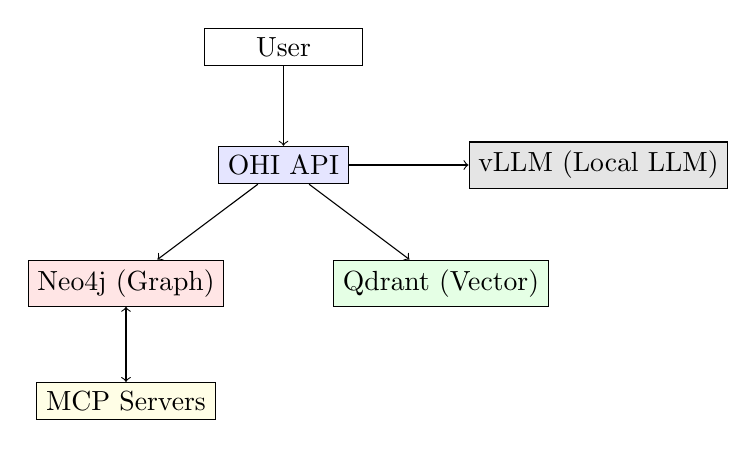
\begin{tikzpicture}[node distance=1.5cm]
        \node[draw, rectangle, minimum width=2cm] (User) {User};
        \node[draw, rectangle, fill=blue!10, below of=User] (API) {OHI API};
        \node[draw, rectangle, fill=red!10, below of=API, xshift=-2cm] (Neo4j) {Neo4j (Graph)};
        \node[draw, rectangle, fill=green!10, below of=API, xshift=2cm] (Qdrant) {Qdrant (Vector)};
        \node[draw, rectangle, fill=yellow!10, below of=Neo4j] (MCP) {MCP Servers};
        \node[draw, rectangle, fill=gray!20, right of=API, xshift=2.5cm] (vLLM) {vLLM (Local LLM)};
        
        \draw[->] (User) -- (API);
        \draw[->] (API) -- (Neo4j);
        \draw[->] (API) -- (Qdrant);
        \draw[->] (API) -- (vLLM);
        \draw[<->] (Neo4j) -- (MCP);
    \end{tikzpicture}
    \caption{High-Level Architecture: The API orchestrates verification across Graph, Vector, and MCP sources using local inference.}
    \label{fig:arch}
\end{figure}

\subsection{Infrastructure Components}
As defined in \texttt{docker-compose.yml}, the system comprises an isolated network of microservices:

\begin{itemize}
    \item \textbf{vLLM (Inference Engine):} Hosts \texttt{Qwen2.5-7B-Instruct-AWQ}. vLLM's *PagedAttention* algorithm manages Key-Value (KV) cache blocks like an operating system, allowing for a 24x higher throughput than naive implementations. This is vital for the parallel nature of claim verification.
    \item \textbf{Neo4j (Ontology Store):} Stores the Wikipedia knowledge graph. It provides "index-free adjacency," enabling swift multi-hop traversals required for complex structural validation.
    \item \textbf{Qdrant (Semantic Store):} Hosts high-dimensional embeddings. Used for the initial, fuzzy retrieval of factual candidates before graph-based refinement.
    \item \textbf{Redis (Cache):} Provides ephemeral storage for frequent claim lookups to reduce repeated inference latency.
\end{itemize}

\subsection{Verification Engine: Qwen 2.5}
We employ Qwen 2.5 (7B and 32B variants) as our primary verification agent. Its excellence in generating structured JSON output is critical for stable claim decomposition. Furthermore, its support for a 128k token context window allows for the ingestion of long-form documentation as a referential context during the verify-loop.

\subsection{The Model Context Protocol (MCP)}
A critical innovation in OHI is the use of the \textbf{Model Context Protocol (MCP)} to standardize data access. Traditionally, integrating fragmented data sources (SQL, Knowledge Graphs, APIs) required brittle, proprietary "Connectors." MCP addresses this through a standardized client-server architecture using JSON-RPC 2.0.

\subsubsection{MCP vs. LangChain}
While LangChain is an excellent framework for orchestrating "how the agent thinks," MCP focuses on "what the agent can access." 
\begin{table}[h]
\centering
\caption{Architectural Comparison: MCP vs. LangChain}
\begin{tabular}{@{}lll@{}}
\toprule
\textbf{Feature} & \textbf{MCP} & \textbf{LangChain} \\ \midrule
Type & Protocol/Standard & Framework/Library \\
Focus & Universal Connect. & Orchestration \\
Security & Process Isolation & Shared Environment \\
Role in OHI & Ground Truth Access & Control Logic \\ \bottomrule
\end{tabular}
\end{table}

\subsubsection{The Sidecar Pattern \& SSE}
The \texttt{mcp\_wikipedia.py} adapter functions as a sidecar service, establishing persistent connections to MCP servers via Server-Sent Events (SSE). To minimize the overhead of SSE handshakes, we implement the \texttt{MCPSessionPool}, maintaining a pool of active \texttt{sse\_client} sessions. This ensures sub-millisecond query latency for repeated verification requests.

\section{Algorithmic Core: The Hybrid Oracle}

The heart of OHI is the \texttt{HybridVerificationOracle}, which implements a multi-strategy pattern to determine truth across structured and unstructured sources.

\subsection{End-to-End Verification Pipeline}
The transformation from a raw LLM output to a verified text with a trust score follows a rigorous pipeline:
\begin{enumerate}
    \item \textbf{Input:} A user query is processed by the generative LLM (e.g., Qwen 2.5 via vLLM).
    \item \textbf{Response Generation:} The model generates a candidate response $R$.
    \item \textbf{Decomposition:} A specialized "Critic-Agent" decomposes $R$ into an array of $n$ atomic claims $A = \{c_1, \dots, c_n\}$ in JSON format.
    \item \textbf{Verification (Parallel):} For each claim $c_i$:
        \begin{itemize}
            \item \textbf{Graph Matching:} Search Neo4j for exact path existence.
            \item \textbf{Vector Retrieval:} Fetch the $k$ most similar chunks from Qdrant.
            \textbf{MCP Oracle:} Query live external sources (Wikipedia/Context7) for direct evidence.
        \end{itemize}
    \item \textbf{Classification:} Claims are categorized as \textit{Supported}, \textit{Contradicted}, or \textit{Unverifiable}.
    \item \textbf{Scoring:} The \textit{WeightedScorer} aggregates these signals into a final OHI Trust Score.
    \item \textbf{Output:} The text is returned with a visual overlay (Green/Red/Gray) indicating the factuality of each sentence.
\end{enumerate}

\subsection{The Verification Algorithm}
Algorithm \ref{alg:verify} formalizes the scoring logic.

\begin{algorithm}
\caption{Hybrid Verification Protocol}
\label{alg:verify}
\begin{algorithmic}[1]
\State $Score_{total} \gets 0$
\For{each claim $c \in A$}
    \State $E_{graph} \gets \text{Neo4j}.match(c.S, c.P, c.O)$
    \State $E_{vec} \gets \text{Qdrant}.search(embedding(c), k=3)$
    \State $E_{mcp} \gets \text{MCP}.query(c)$
    
    \State $S_{graph} \gets (1.0 \text{ if } E_{graph} \text{ else } 0.0)$
    \State $S_{vec} \gets \text{CosineSimilarity}(E_{vec})$
    
    \State $Trust(c) \gets \alpha S_{graph} + \beta S_{vec} + \gamma S_{mcp}$
    \State $Score_{total} \gets Score_{total} + Trust(c)$
\EndFor
\State \Return $Score_{total} / |A|$
\end{algorithmic}
\end{algorithm}

\subsection{Scoring Weights}
The \texttt{WeightedScorer} applies non-linear weighting:
\begin{itemize}
    \item \textbf{Graph Exact Match ($\alpha = 0.6$):} Represents deterministic truth.
    \item \textbf{Vector Semantic Match ($\beta = 0.3$):} Indicates plausibility.
    \item \textbf{MCP Evidence ($\gamma = 0.1$):} Provides contextual grounding.
\end{itemize}

\section{Data Ingestion \& Ground Truth}
A verification system is only as good as its reference data. OHI utilizes a robust ETL pipeline (\texttt{import\_wikipedia\_to\_neo4j.py}) to construct its "Ground Truth."

\subsection{Dynamic Knowledge Graphs (DKG)}
A static graph is insufficient in a volatile world. OHI moves towards \textbf{Dynamic Knowledge Graphs} that reflect temporal and evolving truths:
\begin{itemize}
    \item \textbf{Temporal Dimension:} Facts have a lifespan. Edges in Neo4j are tagged with $t_{valid}$ timestamps. Algorithms for \textit{Temporal Knowledge Graph Completion} (TKGC) are used to predict the current validity of facts and detect temporal inconsistencies.
    \item \textbf{Automated Construction:} Manual curation is non-scalable. We utilize LLM-driven ingestion pipelines that extract triples from unstructured data streams (news feeds, logs) to update the graph in real-time.
\end{itemize}

\subsection{Streaming XML Parsing \& Ontological Mapping}
Processing massive datasets like the Wikipedia XML dump (>20GB) requires memory-efficient streaming. Using \texttt{iterparse}, the system clears elements immediately after processing. During mapping, raw text is transformed into:
\begin{itemize}
    \item \textbf{Categories:} Mapping Wiki-Markup categories to \texttt{[:IN\_CATEGORY]} edges.
    \item \textbf{Internal Links:} Mapping hyperlinks to \texttt{[:LINKS\_TO]} edges, creating a traversable semantic topology.
\end{itemize}
This structured ingestion ensures that every link in the original source becomes a logical path for the verification oracle.

\subsection{Batch Processing \& Resilience}
To handle the scale (millions of nodes), the importer implements:
\begin{itemize}
    \item \textbf{Batch Commit:} Transactions are grouped (e.g., 5000 nodes) to optimize Neo4j write performance.
    \item \textbf{Checkpointing:} The script saves the \texttt{last\_page\_id}. If the Docker container crashes, it resumes exactly where it left off, ensuring data integrity without full re-runs.
\end{itemize}

\section{Performance \& Implementation Analysis}

\subsection{Hardware Requirements}
Running OHI in "Sovereign Mode" imposes specific hardware constraints, primarily dictated by the LLM and Knowledge Graph size.
\begin{table}[h]
\centering
\caption{Infrastructure Requirements for OHI Node}
\begin{tabular}{@{}ll@{}}
\toprule
\textbf{Component} & \textbf{Requirement} \\ \midrule
LLM (Qwen2.5-7B-AWQ) & 8GB VRAM (GPU) \\
Embedding Model & 1GB VRAM / 2GB RAM \\
Neo4j (Graph) & 4GB--16GB RAM \\
Qdrant (Vector) & 4GB RAM (per 1M vectors) \\
\textbf{Total System} & \textbf{min. 16GB RAM + NVIDIA GPU} \\ \bottomrule
\end{tabular}
\end{table}

\subsection{Latency \& Implementation Bottlenecks}
The current implementation is Python-dominated, which introduces a performance ceiling. While sub-millisecond latencies are achieved for database queries (Neo4j/Qdrant), the orchestration and claim decomposition (LLM inference) remain bottlenecks.
\begin{itemize}
    \item \textbf{Decomposition:} ~200--500ms per text segment.
    \item \textbf{Concurrent Orchestration:} Asynchronous Python tasks handle parallel check, but CPython's GIL and I/O overhead kumulativly create delays.
\end{itemize}
Future iterations toward a production-grade system will likely involve porting the core orchestration and embedding computation to \textbf{Rust}. This would allow for native speed in parallel vector and graph queries, reducing verification latency to near real-time levels.

\section{Discussion}

\subsection{OHI as Instrument of Governance and Compliance}
With regulations like the EU AI Act, the need for verifiable accuracy is paramount. OHI transforms "vague safety" into a quantifiable KPI.
\begin{itemize}
    \item \textbf{Auditability:} Since OHI is grounded in deterministic graphs, every trust score is traceable to specific source provenance.
    \item \textbf{Risk Management:} Organizations can enforce thresholds (e.g., "Discard answers with OHI < 0.8"), enabling LLM deployment in high-stakes environments like medicine or finance.
\end{itemize}

\subsection{Limitation: The Entity Linking Challenge}
A significant bottleneck remains the mapping of text spans to graph nodes (\textit{Entity Linking}). Ambiguities (e.g., "Paris" referring to the city vs. the mythological figure) can cause verification collapse. We are exploring \textbf{Generative Entity Linking}, using the LLM's own latent knowledge to disambiguate context before performing the graph lookup.

\subsection{The Future: LLMs as "Gardeners of the Graph"}
We envision a recursive architecture where LLMs serve not only as consumers but as producers of Ground Truth. In this paradigm, "LLMs as Gardeners" extract triples from new, unverified texts to update the Neo4j ontology via MCP. OHI then monitors the same models using the structure they helped build. This creates a self-correcting feedback loop, though it raises critical questions regarding the ultimate authority of truth: \textit{Who owns the graph?}

\subsection{Epistemological Sovereignty}
By relying on local models and open data dumps (Wikipedia), OHI addresses the geopolitical risk of AI. Proprietary models like GPT-4 are "black boxes" whose training data and biases are opaque. OHI allows an organization to define its own "Truth"—whether that is Wikipedia, internal corporate documentation (via \texttt{Context7}), or a scientific paper repository. The definition of truth becomes a configurable parameter of the system, not a hidden variable of the model provider.

\subsection{The "Context7" Use Case: Domain Specificity}
The inclusion of \texttt{mcp\_context7.py} highlights a crucial capability: \textbf{Domain-Specific Verification}.
While Wikipedia verifies general facts ("When was Einstein born?"), specialized domains (e.g., software engineering) require dynamic truth. A library version might change overnight. The Context7 adapter demonstrates how OHI can plug into live documentation streams.
\begin{itemize}
    \item \textit{Claim:} "React useMemo requires a dependency array."
    \item \textit{Verification:} OHI queries the Context7 MCP server, which retrieves the latest React docs.
    \item \textit{Result:} Truth is established against the \textit{current} version of the software, not the version present in the LLM's training cutoff.
\end{itemize}

\section{Future Work}

\subsection{Automated Graph Construction}
Currently, the graph is built from explicit Wikipedia structure. Future work involves using the LLM itself to extract relationships from unstructured text during ingestion ("LLM as Knowledge Engineer"), effectively allowing the system to expand its own ontology.

\subsection{Real-Time Stream Verification}
Adapting the architecture to process live audio transcripts or video feeds. This would require porting the core logic from Python to Rust (using bindings for Neo4j and Qdrant) to meet real-time constraints (< 100ms latency).

\section{Conclusion}
The Open Hallucination Index marks the transition from the era of "Plausible AI" to "Verifiable AI." By decoupling generation from verification and utilizing a sovereign architecture of Graphs, Vectors, and MCP, we provide the blueprints for an epistemic "Trust Layer." In a world where the cost of generating misinformation is near zero, the capability for verifiable truth becomes the most valuable asset in the digital ecosystem.

\begin{thebibliography}{12}
    \bibitem{bender2021} Bender, E. M., Gebru, T., McMillan-Major, A., \& Shmitchell, S. (2021). "On the Dangers of Stochastic Parrots: Can Language Models Be Too Big?". \textit{ACM Conference on Fairness, Accountability, and Transparency (FAccT)}.
    \bibitem{jaeger2024} Jäger, T. (2024). "Epistemic authority and generative AI in learning spaces: rethinking knowledge in the algorithmic age". \textit{Frontiers in Education}.
    \bibitem{min2023} Min, S., Krishna, K., Lyu, X., Lewis, M., Yih, W., Koh, P., \& Iyyer, M. (2023). "FActScore: Fine-grained Atomic Evaluation of Factual Precision in Long Form Text Generation". \textit{EMNLP}.
    \bibitem{pan2024} Pan, L., Zhang, J., Ouyang, L., \& Wang, W. (2024). "Unifying Large Language Models and Knowledge Graphs: A Roadmap". \textit{IEEE Transactions on Knowledge and Data Engineering}.
    \bibitem{lewis2020} Lewis, P., et al. (2020). "Retrieval-Augmented Generation for Knowledge-Intensive NLP Tasks". \textit{NeurIPS}.
    \bibitem{mcp2024} Anthropic. (2024). "Model Context Protocol (MCP) Specification". \textit{https://modelcontextprotocol.io}.
    \bibitem{lettria2024} Lettria. (2024). "VectorRAG vs. GraphRAG: a convincing comparison". \textit{https://lettria.com}.
    \bibitem{motoki2024} Motoki, F., Neto, R. P., \& Rodrigues, V. (2024). "Is ChatGPT conservative or liberal?". \textit{Political Science Research and Methods}.
    \bibitem{espejel2023} Espejel, J., et al. (2023). "GPT-4, GPT-3.5 and the political bias of generative AI". \textit{arXiv preprint arXiv:2305.14251}.
    \bibitem{shah2024} Shah, S., et al. (2024). "ReDeEP: Detecting Hallucination in Retrieval-Augmented Generation via Mechanistic Interpretability". \textit{arXiv preprint arXiv:2409.03571}.
    \bibitem{vaswani2017} Vaswani, A., et al. (2017). "Attention Is All You Need". \textit{NeurIPS}.
    \bibitem{qwen2024} Qwen Team. (2024). "Qwen2.5: A Party of Foundation Models". \textit{Alibaba Cloud}.
\end{thebibliography}

\end{document}